\documentclass{uopThesis}



\usepackage[authoryear,comma]{natbib}



\title{Thesis title}

%% The full name of the author
\author{ Student Name }
%% The full name of your supervisor
\supervisor {Supervisor name }

\dept{Department of Statistics and Computer Science}

\university{University of Peradeniya}

\degree{Your degree program}%% BSc.(Hons) in Computer Science


\begin{document}
	
\maketitle 
\frontmatter
 \begin{abstract}
	

	
	This is where you write your abstract ...All the pages in the Project Report/Thesis must be computer printed only on one side of the page using
	Times New Roman (size 12) font with 1.5-line spacing.
	
	
\end{abstract}

 \addcontentsline{toc}{chapter}{ABSTRACT}
 
 \begin{declaration}      
	
	
I do hereby declare that the work reported in this research thesis was exclusively carried out by me under the supervision of {Name of the supervisor}. It describes the results of my own independent word except where due reference has been made in the text. No part of this research thesis has been submitted earlier or concurrently for the same or any other degree.
	
	
\end{declaration}
 \addcontentsline{toc}{chapter}{DECLARATION}
 
 \begin{acknowledgement}      
	
	
	And I would like to acknowledge ...
	
	
\end{acknowledgement}
 \addcontentsline{toc}{chapter}{ACKNOWLEDGEMENT} 

\addcontentsline{toc}{chapter}{TABLE OF CONTENTS}

\addcontentsline{toc}{chapter}{LIST OF FIGURES}

\addcontentsline{toc}{chapter}{LIST OF TABLES}

\tableofcontents

\cleardoublepage
\listoftables
\cleardoublepage
\listoffigures
\mainmatter
\doublespacing

% add chapters here
\chapter{Introduction}  %Title of the First Chapter

%\ifpdf
%\graphicspath{{Chapter1/Figs/Raster/}{Chapter1/Figs/PDF/}{Chapter1/Figs/}}
%\else
%\graphicspath{{Chapter1/Figs/Vector/}{Chapter1/Figs/}}
%\fi


%********************************** %First Section  **************************************
\section{Problem Statement} %Section - 1.1 

 

 

All the pages in the Project Report/Thesis must be computer printed only on one side of the page using
Times New Roman (size 12) font with 1.5-line spacing.
However, the following components of the project report/thesis should have single-line spacing: declaration, abstract, acknowledgment, table of contents, list of tables, list of figures, list of abbreviations, table titles, figure captions, and references. 
Each reference must be separated by a single-line spacing. Margins on each page must be maintained as
follows: left hand, 40 mm; right hand, 15 mm; top and bottom, 25 mm.  
\citep{Streftaris2004} 

%% this is how you can add images
\section{Outline of Thesis}
\begin{figure}[h!]
  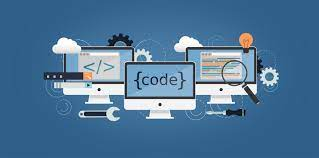
\includegraphics[width=\linewidth]{images/image.jpg}
  \caption{Computer Science}
  \label{fig: computer science}
\end{figure}
 

\chapter{Literature Review}  %Title of the First Chapter

\section{Section 1} %Section - 1.1 

 

 

your literature review goes here........... 


\chapter{Methodology}  %Title of the First Chapter

\section{Section 1} %Section - 1.1 

 
This is where you write your methodology ...
\chapter{Results and discussion}  %Title of the First Chapter

\section{Section 1} %Section - 1.1 

This is where you write your results and discussion ...
\chapter{Conclusion}  %Title of the First Chapter

\section{section 1} %Section - 1.1 

This is where you write your conclusion ...

 


%\bibliographystyle{apalike}
%\bibliographystyle{unsrt} % Use for unsorted references  
%\bibliographystyle{plainnat} % use this to have URLs listed in References
 
\cleardoublepage
\bibliographystyle{apalike}%apalike}%agsm} 
\bibliography{References.bib}   % Path to your References.bib file	
	
\end{document}
